\documentclass[11pt,letterpaper]{article}
\usepackage[utf8]{inputenc}

%----- Configuración del estilo del documento------%
\usepackage{epsfig,graphicx}
\usepackage[left=2cm,right=2cm,top=1.8cm,bottom=2.3cm]{geometry}
\usepackage{fancyhdr}
\usepackage{lastpage}

\usepackage{xcolor}
\usepackage{soul}
\newcommand{\mathcolorbox}[2]{\colorbox{#1}{$\displaystyle #2$}}

\usepackage{float}

% \usepackage{cite}
\usepackage{multicol}
\setlength{\columnsep}{1.5cm}
\setlength{\columnseprule}{.5pt}

\pagestyle{fancy}
\fancyhf{}
\rfoot{\textit{Página \thepage \hspace{1pt} de \pageref{LastPage}}}

%------ Paquetes matemáticos básicos --------%
\usepackage{amsmath}
\usepackage{amssymb}
\usepackage{amsthm}

%------ Paquetes para codigo --------%
\usepackage{tikz}

%------ Paquetes para citar --------%
\usepackage[spanish]{babel}
\usepackage{csquotes} % Recomendado para biblatex
% Carga biblatex con estilo APA; asegúrate de usar biber como backend.
\usepackage[backend=biber,style=apa]{biblatex}
\addbibresource{./src/referencias/referencias.bib} % Ruta a tu archivo .bib



\begin{document}

%------ Encabezado -------- %
\begin{center}
    \begin{minipage}{3cm}
    	\begin{center}
    		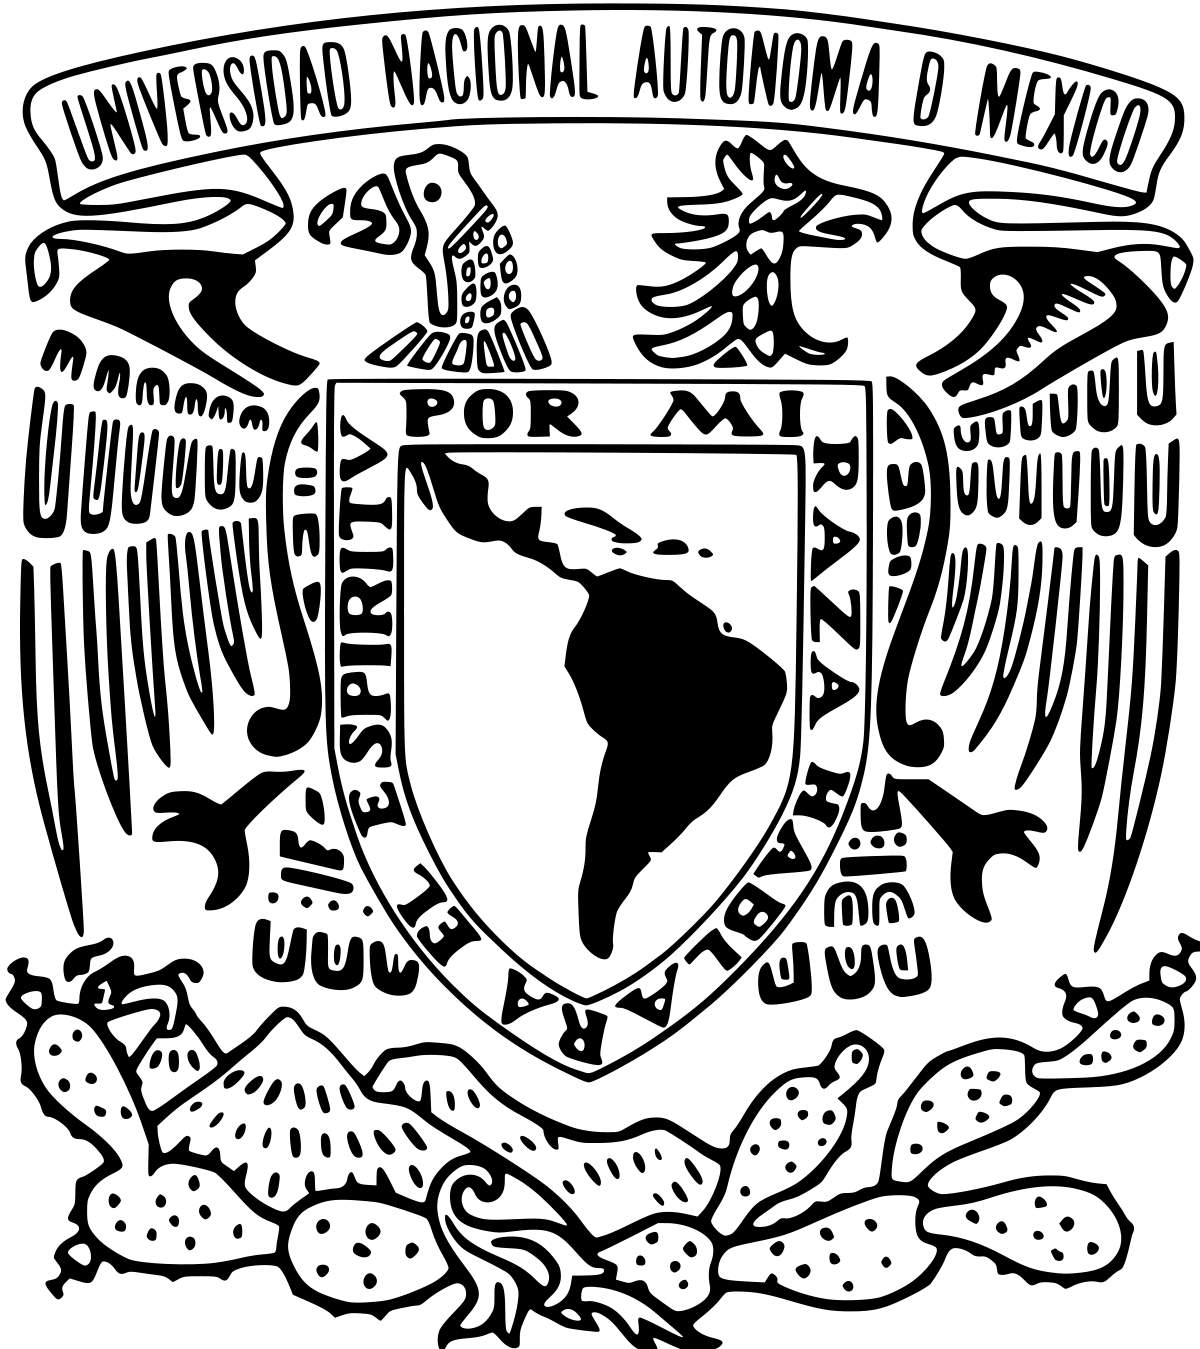
\includegraphics[height=3.2cm]{src/Img/Logo_UNAM.png}
    	\end{center}
    \end{minipage}\hfill
    \begin{minipage}{10cm}
    	\begin{center}
    	\textbf{\large Universidad Nacional Autónoma de México}\\[0.1cm]
        \textbf{Facultad de Ciencias}\\[0.1cm]
        \textbf{Inteligencia Artificial $|$ 7003}\\[0.1cm]
        Examen Parcial 1 $|$ Introducción y Agentes \\[0.1cm]
        Sosa Romo Juan Mario $|$ 320051926 \\[0.1cm]
        24/02/24
    	\end{center}
    \end{minipage}\hfill
    \begin{minipage}{3cm}
    	\begin{center}
    		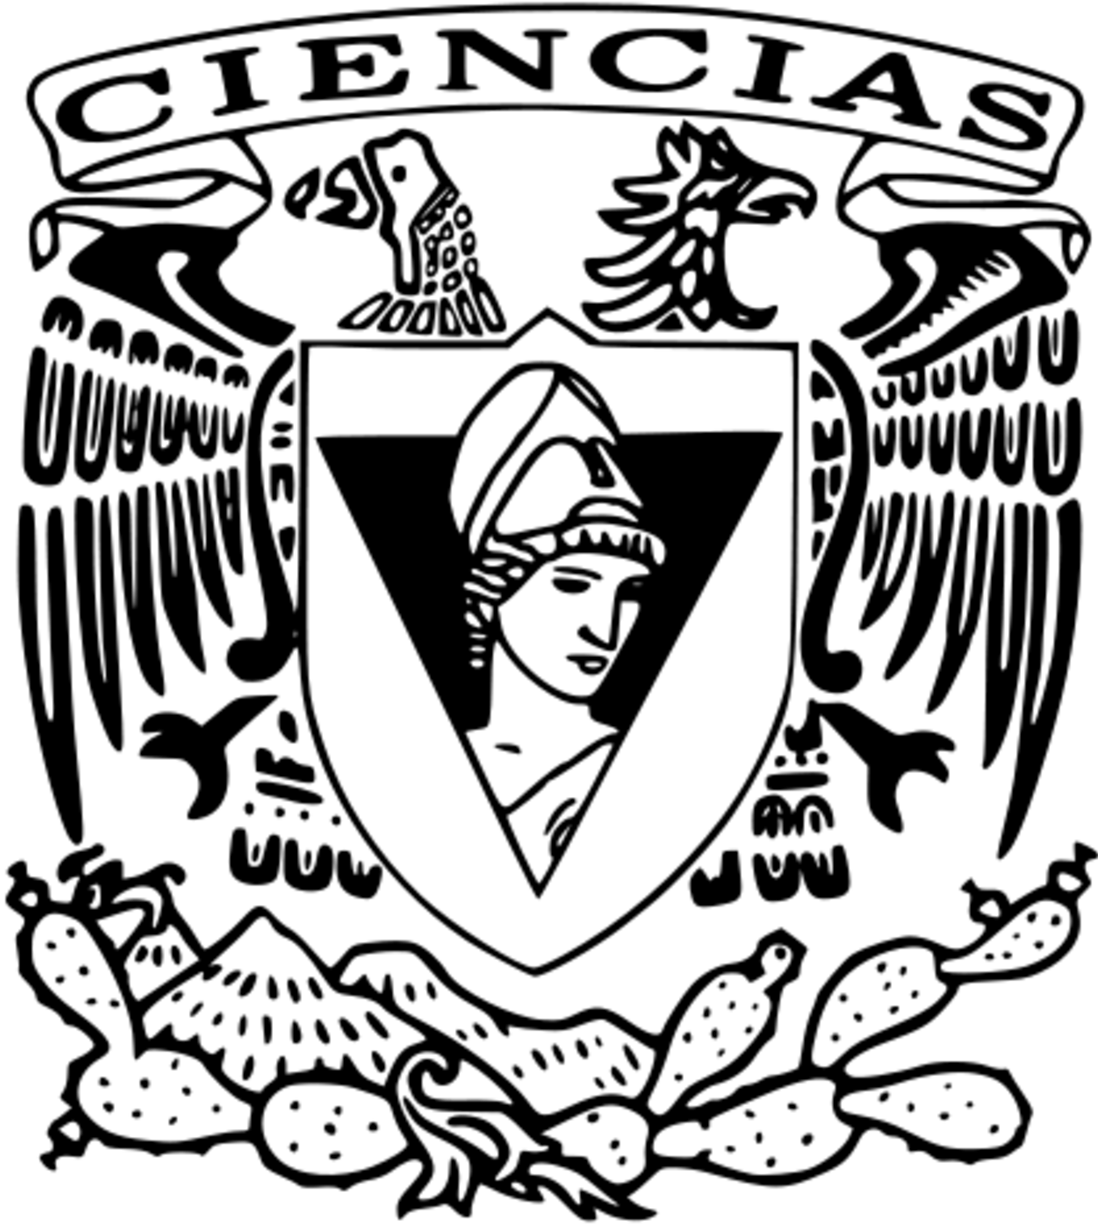
\includegraphics[height=3.2cm]{src/Img/Logo_FC.png}
    	\end{center}
    \end{minipage}
\end{center}


\rule{16.9cm}{0.1mm}
\vspace{0.3cm}

\vspace{0.3cm}
%------ Ejercicios -------- %
\begin{enumerate}
    \item \textbf{Ejercicio 1.} (25 pts.) Evalúa las siguientes expresiones usando las téctnicas de paso de prámetros que se indican. En cada caso debes mostrar cómo queda el ambiente y memoria final, tal y como se vio en clase. \vspace{0.3cm}

\begin{itemize}
    \item Evalúa el siguiente código bajo paso por valor y por referencia.
\begin{lstlisting}
(let [(list1 (box '(1 2 3)))
    (list2 (box '(4 5 6)))
    (concat-lists (lambda (x y)
                    (begin
                        (set! x (append (unbox x) (unbox y)))
                        (set! y '(0)))))]
    (begin
        (concat-lists list1 list2)
        (list (unbox list1) (unbox list2))))
\end{lstlisting}

    \item Evalúa el siguiente código bajo paso por nombre y por necesidad.
\begin{lstlisting}
(let [(acc 0)
    (conditional (lambda (x)
                    (if (> x 0)
                        (begin (set! acc (+ acc 1)) acc)
                        (begin (set! acc (- acc 1)) acc))))
    (compute (lambda (y) (* y y)))]
(compute (conditional acc)))
\end{lstlisting}
\end{itemize}



    \item \textbf{Explica los tres paradigmas principales de la I.A., así como sus características principales (1 pt.).}

\begin{itemize}
    \item \textbf{Simbólico}
    
    En esencia, este enfoque busca conseguir "inteligencia" mediante el uso de símbolos y reglas. Es útil si queremos hacer cosas más determinísticas o más estructuradas. \vspace{.3cm}

    Es un enfoque más limitado en términos de escalabilidad, pues se tiene que, de cierta forma, saber de manera previa lo que se quiere que el sistema sepa. \vspace{.3cm}
    
    \cite{russell2020artificial}

    \item \textbf{Estadístico}
    
    Como su nombre lo indica, este paradigma se apoya en métodos probabilísticos y estadísticos, como la regresión, para intentar corregir o determinar la incertidumbre. Incluye métodos como los de aprendizaje supervisado, no supervisado y de refuerzo. \vspace{.3cm}

    En sí, son bastante útiles para detectar patrones en grandes cantidades de datos y se aplican en modelos económicos o en los conocidos algoritmos de redes sociales. \vspace{.3cm}

    En esencia, este enfoque presenta dos problemas principales. El primero, y el más grande (no solo para este tipo de IA), es la cantidad y calidad de los datos; al tratarse de modelos diseñados para procesar grandes volúmenes de información, conseguir datos y verificar que sean válidos es complicado. El segundo problema es el de la caja negra: a diferencia del enfoque anterior, en el que los procesos son relativamente más simples de entender y simular, en este paradigma, al no ser necesario mostrar o explicar cada paso sino solo el resultado y el modelo, se vuelve bastante más complejo comprender su funcionamiento. \vspace{.3cm}

    \cite{bishop2006pattern}

    \item \textbf{Neuronal}
    
    Finalmente, tenemos el paradigma neuronal. Como su nombre lo indica, esta corriente se basa en el funcionamiento de los cerebros orgánicos, especialmente el de los humanos; en su núcleo se plantea la idea de computar a través de una red de unidades independientes distribuidas, que reciben una serie de señales y generan otra serie de señales tras procesarlas. \vspace{.3cm}

    Además de las unidades, denominadas neuronas, existen capas de entrada, ocultas y de salida, que son agrupaciones de neuronas con comportamientos específicos. Una ventaja de este enfoque es que pierde gran parte de la estructura rígida que requieren los otros dos, volviéndose más flexible y permitiendo enfocarse en las entradas y salidas. Esto, a su vez, implica que nuevamente surge el problema de la caja negra, y en este caso, aún más marcado. \vspace{.3cm}

    Este enfoque es el más popular actualmente, a mi parecer, por su gran escalabilidad; además, estos modelos son capaces de tratar con datos no estructurados, lo que los hace mucho mejores en tareas de traducción o procesamiento de imágenes. \vspace{.3cm}

    \cite{goodfellow2016deep}
\end{itemize}

Finalmente, me gusta agregar que, aunque son tres enfoques diferentes, en la práctica es muy común utilizar una combinación para aprovechar las ventajas de cada uno y compensar las limitaciones de los otros.

    \item \textbf{Ejercicio 3.} (25 pts.) Realiza el juicio de tipo para cada una de las siguientes expresiones, usa las reglas vistas en clase o define una nueva regla en caso de ser necesario. Observa que la primera expresión no tiene anotaciones de tipo, por lo que tendras que definir las reglas para verificar los tipos. \vspace{0.3cm}

\begin{enumerate}
\item 
\begin{lstlisting}
(let (g (lambda (x) (x 4)))
    (g (lambda (y) (-y 2))))
\end{lstlisting}

\item 
\begin{lstlisting}
(letrec (f : number -> number
    (fun (x : number) : number
        (if0 x 1 (* n (f (- n 1))))))
    (f 5))
\end{lstlisting}
\end{enumerate}
    \item \textbf{Investiga y explica brevemente de qué se trata el juego de la imitación de Alan M. Turing. Cita tus fuentes (0.5 pt.).}

También conocido como la prueba de Turing, es un experimento mental propuesto por Alan M. Turing en su artículo \textit{Computing Machinery and Intelligence}. La idea es que, para probar la consciencia o su ausencia en las máquinas, se sitúan una máquina, una persona y una segunda persona que actuará como juez; de esta forma, mediante preguntas y respuestas, el mediador, representado en la figura 'C', debe determinar quién es la computadora y quién es la persona. Si el sistema es capaz de engañar a un alto porcentaje de los jueces, se le considera que ha pasado la prueba de Turing. \vspace{.3cm}

\cite{turing1950computing}

\begin{figure}[h]
    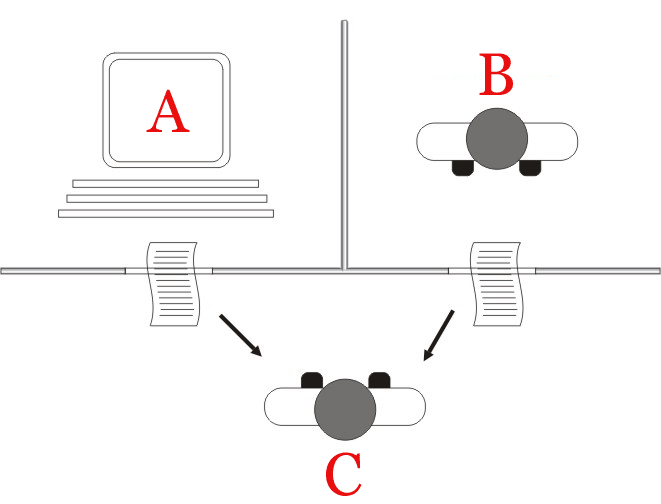
\includegraphics[width=10cm]{src/Img/Turing_test_diagram.png}
    \centering
    \caption{\cite{testTuring}}
\end{figure}

Aunque el hecho de que el sistema pase el test, en realidad, no nos indica más que su capacidad para comunicarse de manera coherente. Aun así, es altamente probable que nos encontremos ante un escenario similar al experimento del cuarto chino de John Searle, en el que la computadora realmente no tiene idea de lo que está haciendo, pero es capaz de engañar al mediador mediante tácticas inteligentes, generalmente basadas en métodos estadísticos y neuronales. \vspace{.3cm}

    \item \textbf{Investiga en qué informe se declara el fracaso del programa de traducción de máquina, y explica brevemente las razones que en él se esbozan. Cita tus fuentes (1 pt.).}

El informe al que se refiere la pregunta es el elaborado por el \textit{Automatic Language Processing Advisory Committee} (ALPAC) en 1966, donde se revisaron los avances en este tipo de inteligencia artificial y se concluyó que los resultados no eran satisfactorios, recomendándose redirigir el enfoque y los recursos hacia otras áreas de investigación. \vspace{.3cm}

De manera sencilla, el programa fracasó porque no era capaz de generar traducciones de buena calidad, especialmente en comparación con aquellas realizadas por traductores profesionales. Además, se mencionaron grandes limitaciones tanto en hardware como en software de la época, y se destacó que el lenguaje natural es demasiado ambiguo y complejo. En esencia, al comparar los resultados obtenidos con la inversión realizada, el proyecto resultaba insostenible. Este fracaso marcó el inicio del primer "invierno de la IA", lo que redujo significativamente el financiamiento para la investigación en el área, además de que los métodos disponibles no eran lo suficientemente avanzados. \vspace{.3cm}

\cite{alpac1966machine}

    \item \textbf{Explica brevemente qué es un agente racional en el contexto de inteligencia artificial. Preferiblemente incluye un diagrama en tu descripción (1 pt.).}\vspace{.3cm}

Un agente racional es una entidad que busca maximizar su función de utilidad; existe en un entorno y es capaz de percibirlo con sus sensores y, posteriormente, actúa sobre él mediante sus actuadores. De manera simple, un agente racional es una entidad que realiza las acciones que más sentido tienen para cumplir sus objetivos. \vspace{.3cm}

Para ilustrarlo de manera más gráfica, se incluye un diagrama creado por ICCSI: \vspace{.3cm}

\begin{figure}[H]
    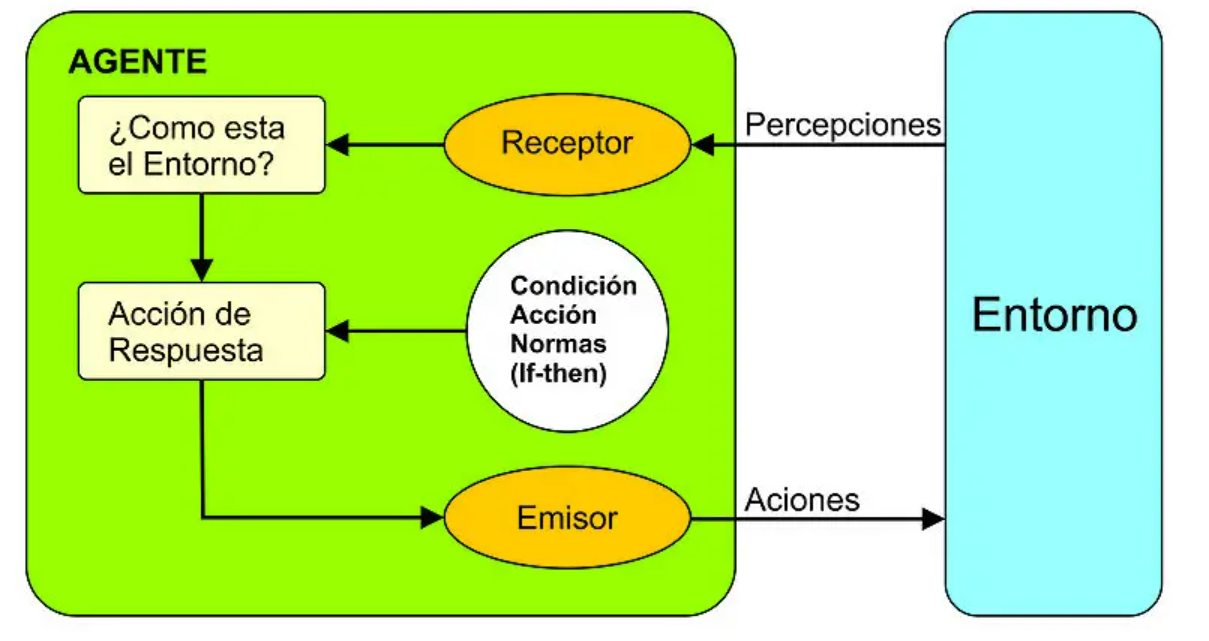
\includegraphics[width=10cm]{src/Img/que-es-un-agente-software-racional-1.png}
    \centering
    \caption{\cite{iccsi_agente_racional_imagen}}
\end{figure}

Como podemos ver, la definición de agente es lo suficientemente amplia para ser utilizada en diversos contextos.

\cite{russell2020artificial}

    \item \textbf{Menciona dos diferencias entre la función de rendimiento y el programa del agente (1 pt.).} \vspace{.3cm}

Como ya sabemos, la función de rendimiento busca evaluar qué tan bien un agente cumple con sus objetivos en su entorno, mientras que el programa del agente se encarga de implementar este comportamiento. Por lo tanto, esta primera diferencia puede compararse con la relación entre teoría y práctica.  

De la misma manera, es evidente que la implementación de la función de rendimiento es independiente del programa del agente; en este sentido, la función representa el \textit{qué} y el programa el \textit{cómo}.  

Finalmente, cabe mencionar que es relativamente más fácil cambiar el programa del agente para mejorar su desempeño, mientras que modificar la función de rendimiento suele ser mucho más complicado. \vspace{.3cm}

    \item \textbf{Considera el mundo de la aspiradora constituido por dos celdas. Si el agente utiliza el siguientealgoritmo para desempeñar sus funciones:}

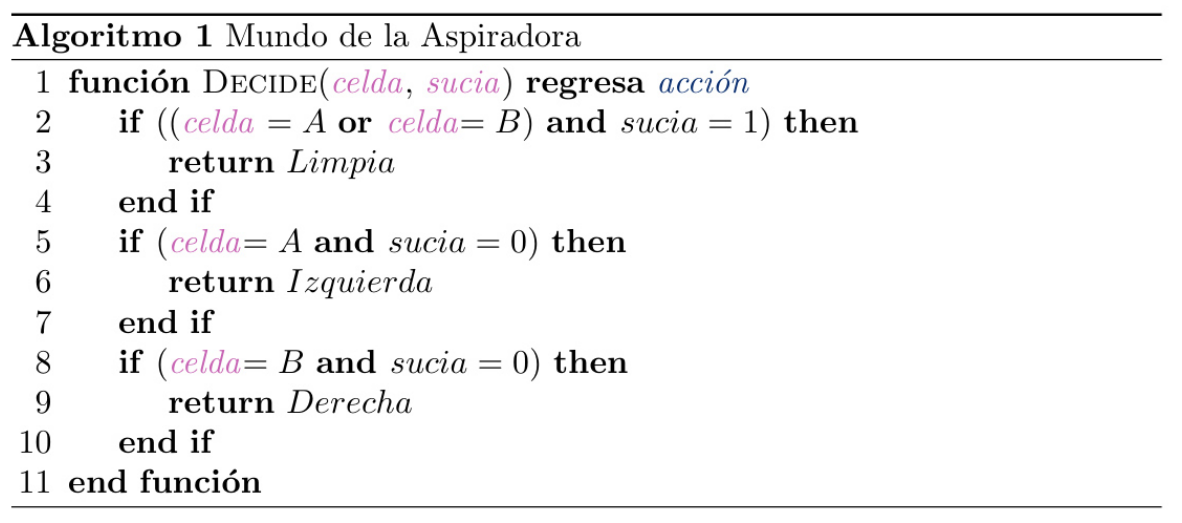
\includegraphics[width=16cm]{src/Img/Screenshot_20250224_024900.png}

indica el tipo de agente en el que podría clasificarse (1 pt.).
    \item \textbf{Menciona tres categorías en las que podemos clasificar los entornos de trabajo (0.5 pt.).}
    \item \textbf{Describe dos situaciones en las que el agente basado en utilidad tiene ventaja sobre el agente basado en objetivo (0.5 pt.).} \vspace{.3cm}

Como menciona~\cite{SotoAstorga2025}, aunque los agentes basados en objetivos son más flexibles que los reactivos simples o con modelo, cuando los objetivos no están bien definidos o no son completamente alcanzables, pueden producir resultados subóptimos. \vspace{.2cm}

Por ejemplo, si quisiéramos diseñar un taxi con IA, este tendría al menos dos objetivos que podrían ser contradictorios entre sí: llegar rápido y llegar seguro. Para un agente basado en objetivos, la contradicción entre estos podría dificultar la toma de decisiones. En cambio, un agente basado en utilidad podría evaluar múltiples rutas y seleccionar aquella que mejor equilibre ambos factores. \vspace{.2cm}

Por lo tanto, en entornos dinámicos o cuando se manejan múltiples objetivos complejos, un agente basado en utilidad ofrece mayor granularidad y precisión en la toma de decisiones en comparación con un agente basado en objetivos.
    \item \textbf{Explica la noción de aprendizaje para agentes (1 pt.).} \vspace{.3cm}

El aprendizaje, no es mas que la capacidad de adaptarse y mejorar sus acciones respecto a su entorno de trabajo, para ello el agente debe obtener experiencia interactuando con su ambiente mediante sus perceptores.

Para procesar y poder \textit{aprender} como tal, se deben acoplar una forma de los siguientes elementos:
\begin{itemize}
    \item \textbf{Critica:} El conocido feedback, es el mecanismo preestablecido que es capaz de darle al agente una manera de saber si sus acciones son las deseadas.
    \item \textbf{Elemento de aprendizaje:} Esta es la parte interesante, pues permite extraer partrones y ajustar la manera en la que el agente toma decisiones en funcion de los resultados obtenidos (critica).
    \item \textbf{Elemento de eficacia:} Esta parte es la que permite al agente tomar la mejor decision para cumplir su objetivo o satisfacer su funcion de utilidad.
    \item \textbf{Generador de problemas:} Maso menos como tu ex (chiste), el generador de problemas literalmente explora sitauciones mas alla de la tarea inmediata para poder explorar situaciones sin tener que exponer el agente fisico a ellas, asi ampliando el conocimiento y evitando estancamiento. 
\end{itemize}

\cite{SotoAstorga2025} \cite{russell2020artificial}
    \item \textbf{Para el mundo de un robot de servicio de cafetería, enuncia: sus sensores, sus efectores, su ambiente, su entorno de trabajo. Además, propón una medida de rendimiento para que su agencia sea racional. Además, indica qué tipo de agente sería mejor implementar para su servicio: basado en modelo, que aprende, dirigido por tabla, o reactivo simple (1 pt.).} \vspace{.3cm}

Primero que nada, estoy considerando un bot como este:

\begin{figure}[H]
    \centering
    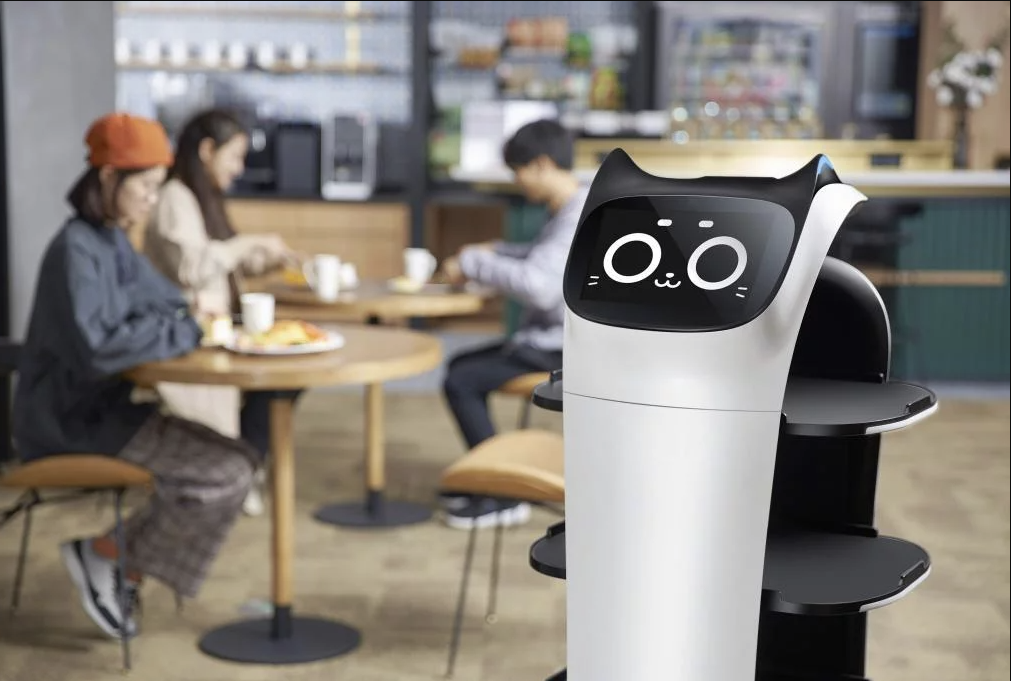
\includegraphics[width=10cm]{src/Img/robot.png}
    \caption{\cite{seboticsImagen}}
\end{figure}

\begin{itemize}
    \item \textbf{Entorno de trabajo:}  
    Voy a comenzar describiendo el tipo de ambiente según las clasificaciones (véase pregunta 9). El ambiente es parcialmente observable, se espera que haya varios agentes interactuando de manera cooperativa, por lo que es un entorno estocástico y muy cambiante. Creo que sería más sencillo tratarlo de manera episódica, con episodios de mayor duración. Además, el entorno es dinámico y se desarrolla de forma continua.
    \begin{itemize}
        \item \textbf{Sensores:}  
        Como mínimo, el robot necesitará cámaras (al menos 3), un velocímetro, algún tipo de pantalla, micrófonos y, quizás, GPS.
        \item \textbf{Efectores:}  
        En este modelo, contará con ruedas, motor, freno, bocina, pantalla y acelerador. No requiere un mecanismo para agarrar el contenido, ya que éste se coloca en sus repisas.
        \item \textbf{Ambiente:}  
        Se trata de una cafetería, con numerosos elementos móviles como sillas, mesas y personas, y algunos elementos estáticos como paredes o estantes.
        \item \textbf{Medida de rendimiento:}  
        Una buena medida de rendimiento podría incluir la rapidez en el servicio, la seguridad en la manipulación de las bebidas, la maximización de ganancias, la reducción de colisiones, el rendimiento de la batería y la satisfacción de los clientes (evaluada mediante encuestas rápidas).
    \end{itemize}
    
    \item \textbf{Tipo de agente:}  
    Considero que el agente debe ser capaz de aprender, ya que sus interacciones con el entorno son complejas. Dado que se enfrenta a un ambiente tan cambiante y con múltiples objetivos, es necesario que sea adaptable. Por ello, se recomienda implementar un agente basado en utilidad, que integre un modelo para poder distinguir lo que está percibiendo y determinar la trayectoria óptima.
\end{itemize}

\end{enumerate}

\printbibliography


\end{document}